\section{The Milestones Project}\label{sec:project}
An early overview of the content and aims of the Milestones Project appeared in \cite{Friendly:04:gfkl}.
Here we update that description and provide a few technical details on some problems in
documenting the history of data visualization in a convenient form for browsing, searching and
analysis.

\subsection{Origin, structure and evolution}\label{sec:structure}
The initial step in portraying the history of data visualization was a simple chronological listing of milestone items
with capsule descriptions, bibliographic references, markers for date, person, place, and links to portraits, images,
related sources or more detailed commentaries.
We started with 105
developments listed by \citet{BenigerRobyn:1978}
and incorporated additional listings from
\citet{Hankins:1999},  \citet{Tufte:1983,Tufte:1990,Tufte:1997},  \citet{Heiser:2000}, and others.

This began as single \LaTeX\ file (with markup tags for all relevant bits of information),
used to produce a
hyper-linked PDF document.  A variety of software tools (perl scripts, Unix utilities) allowed us to turn this
single source
\emph{directly} into the web version originally shown at
\url{http://www.math.yorku.ca/SCS/Gallery/milestone}.  Other custom software tools allowed us to
add new milestones items from text files using a template of tags (DATE:, AUTHOR:, WHAT:, REF:, IMG:, etc.)
and extract the
information about milestones items, authors, images, etc. in a variety of forms (CSV, XML, JSON)
that could be used as input for analyses and graphic displays.  For example, \figref{fig:mileyears4}
was produced in SAS software using a unix command pipe like
\begin{verbatim}
itemdb -o milestones.csv < milestones.tex | sas -i milestones.csv mileyears.sas
\end{verbatim}

It soon became apparent that such a text-based representation was inadequate. Updating the milestones data 
required that the single \LaTeX\ file be shared among several collaborators; milestones 
assets, such as images, web links and references were not easily accessible by others, making collaboration cumbersome. 
Each public release of updates to the web site required steps of verification, re-building and
synchronization with the server.

Around 2005, we began to convert the flat file into a relational database and completely redesign the Milestones 
web site. Specifically, we wanted to facilitate contributions by any number of trusted
collaborators via an easy-to-use web administration area and allow for the dissemination of milestones data 
via an easy-to-browse public user interface, both of which would be tied to the relational database.

Migrating the data to this form provided some challenges. First, the existing milestones data needed to be
normalized and redundancy minimized. To do this, we broke the data into its relevant entities namely the 
milestone itself and its descriptors (aspect, author, subject, keywords, reference, and mediaitem).
The aspect, author, subject, keyword and reference descriptors exist as a many-to-many relationship between 
it and the milestone. For example an aspect can belong to one or more milestones and the milestone can belong to 
one or more aspects. Media items on the other hand, can belong to only one milestone at a time, with
multiple mediaitems possible for a single milestone. \figref{fig:datavis-schema-2} illustrates these relationships.

\begin{figure}[!htb]
  \centering
  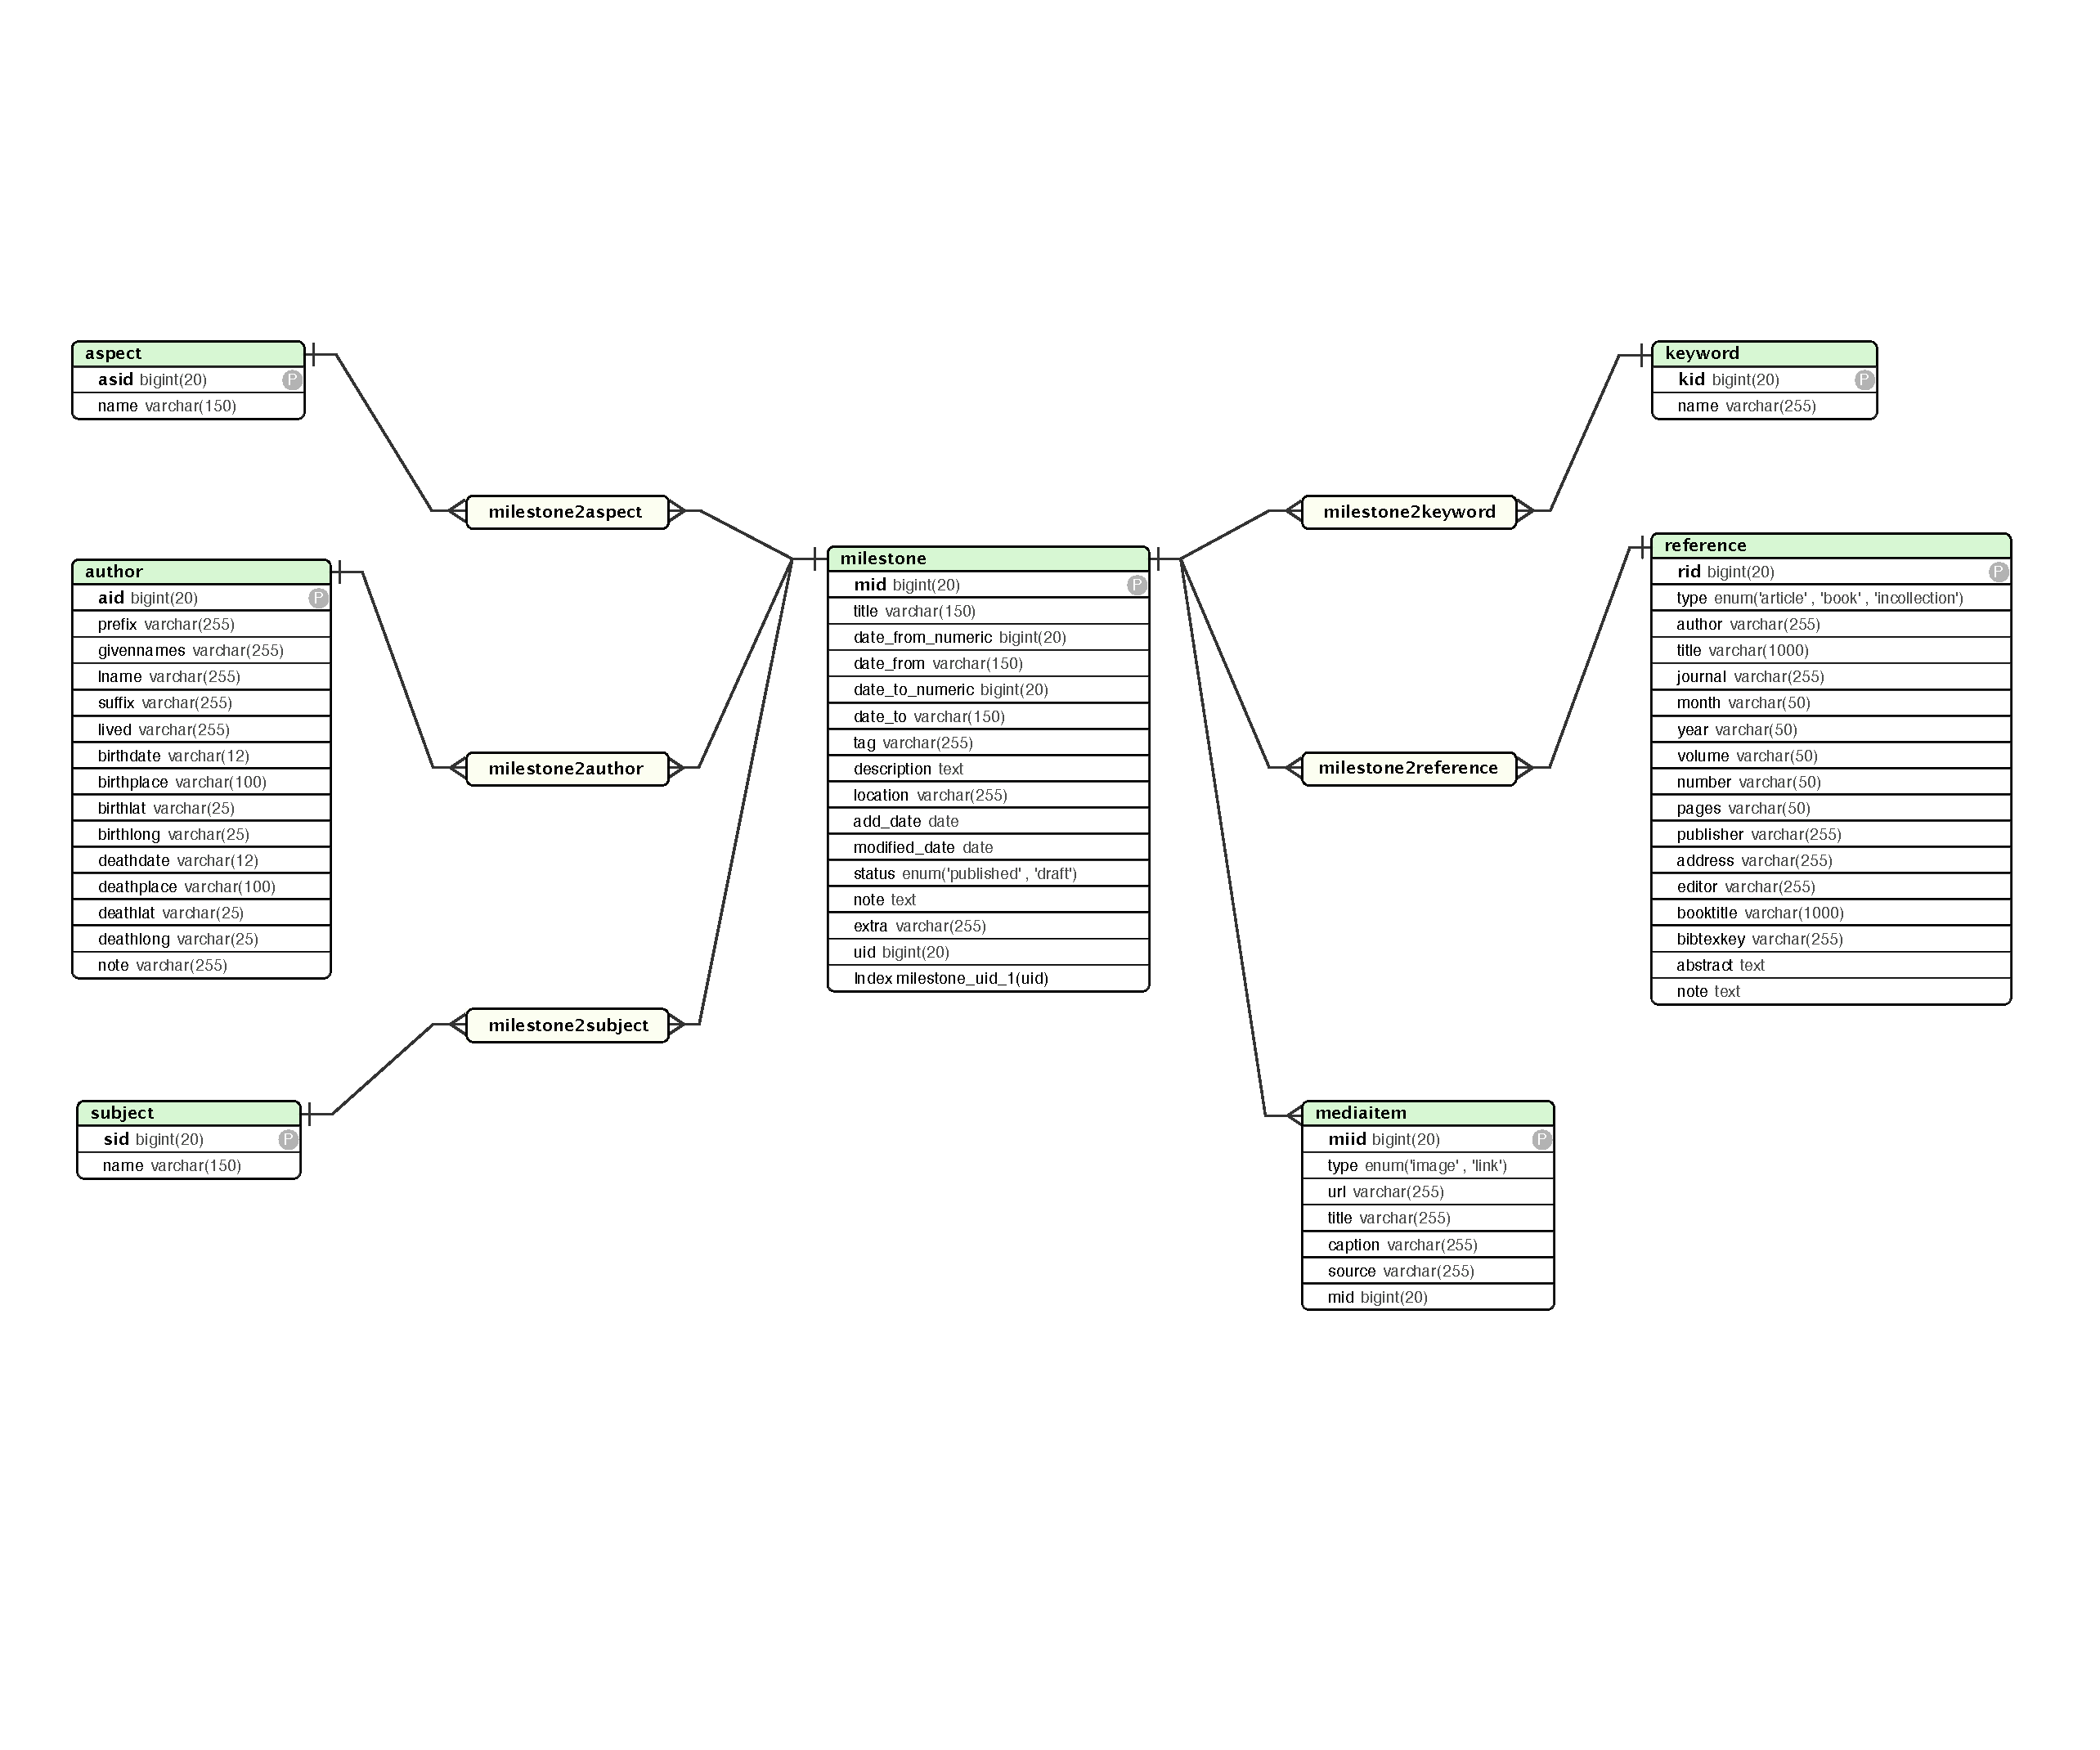
\includegraphics[width=\textwidth,clip]{fig/datavis-schema-2}
  \caption{Simplified schema for the MySQL database for the Milestones Project. The main 
  table (\texttt{milestone}) contains information regarding each of the items considered
  a milestone in the history of data visualization, linked to other tables 
  (e.g., \texttt{reference}, \texttt{mediaitem}) by unique (primary) keys.
  Other supporting tables (e.g., \texttt{milestone2aspect}) provide for convenient lookups of 
  descriptors of these milestones items (\texttt{subject}, \texttt{aspect}, \texttt{keyword}).
  }
  \label{fig:datavis-schema-2}
\end{figure}

Normalizing the data in this way enabled us to free the database of modification anomalies; ensured that the database 
structure was scalable and could be extended with minimum modifications.
Most importantly, it allows for future growth, and provides a query-neutral database model
\citep{Codd:1971} that could be used for web presentation and customized search
on the \url{http://datvis.ca} site, 
as well as for analysis and graphics using milestones data

At present, the Milestones Project lists 288 contributions to this history, with nearly 350 references,
information on 336 authors and 774 media items, comprising 371 images appearing online on the
\url{http://datavis.ca/milestone} site and 403 links to images and documents at other sites.
In addition, we maintain an offline image database comprising over 1100 images collected from
various sources. Over time, we will continue to add these to the online database.

\subsection{User interface}
The second challenge related to how to display such a large amount of information in an easy to understand
user interface to provide overview, search, and details about these events in the history of
data visualization. We decided to retain the time-based grouping of the milestones content by 
epochs (Pre-1600, 1600s, 1700s, etc.), each with a theme (e.g., 1600--1699: Measurement and theory)
and descriptive text.

\begin{figure}[!htb]
  \centering
  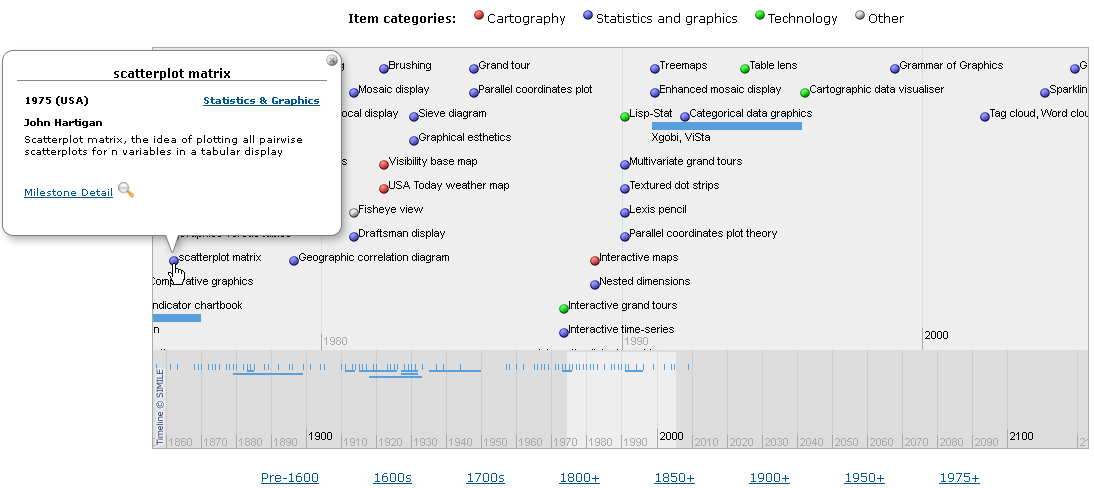
\includegraphics[width=\textwidth,clip]{fig/datavis-timeline2}
  \caption{Timeline view of the Milestones Project on the site \texttt{http://datavis.ca/milestone}. In this view,
  the top panel shows a detailed view of the segment of history highlighted in the bottom panel, both
  of which can be separately scrolled. Items in the top panel show a brief tag, color-coded in coarse
  categories. Clicking on an item in this panel brings up small description, linked to the details of
  the milestone item.
  }
  \label{fig:datavis-timeline2}
\end{figure}

The visual design of the
interface follows Ben Shneiderman's mantra: ``Overview first, zoom and filter, then details on demand''
\citep{Shneiderman:1996:IEEE}.
To do this, 
we added a timeline view (\figref{fig:datavis-timeline2}) of the milestones items displayed on the overview
landing page. This timeline, based on the SIMILE Timeline Widget (\url{http://www.simile-widgets.org/timeline})
allows multiple connected bands, showing events at different resolutions.  Each band can be separately panned
by dragging with the mouse pointer, scroll wheel or keyboard arrow keys.  The top panel shows individual milestone
items with brief text tags and color-coded item categories.
Clicking on an item in this panel brings up small description, linked to the details of the milestone item.

The timeline view, although most obvious, is just one of several possibilities for a visual overview
or interaction with the display of the milestones database to support search and exploration.
The software design of the site, using open-source tool kits, makes it relatively simple to add new
ones.  We illustrate a map-based display in \secref{sec:geography}.



